% asset_id: FAS2EulerianTraversabilityAndRouteInspectionTikZ-002
% asset_type: TikZ
% unit_code: FAS2
% topic_code: FAS2-GRAPH
% topic_id: FAS2EulerianTraversabilityAndRouteInspection
\documentclass[tikz,border=8pt]{standalone}
\usetikzlibrary{positioning,calc}
\begin{document}
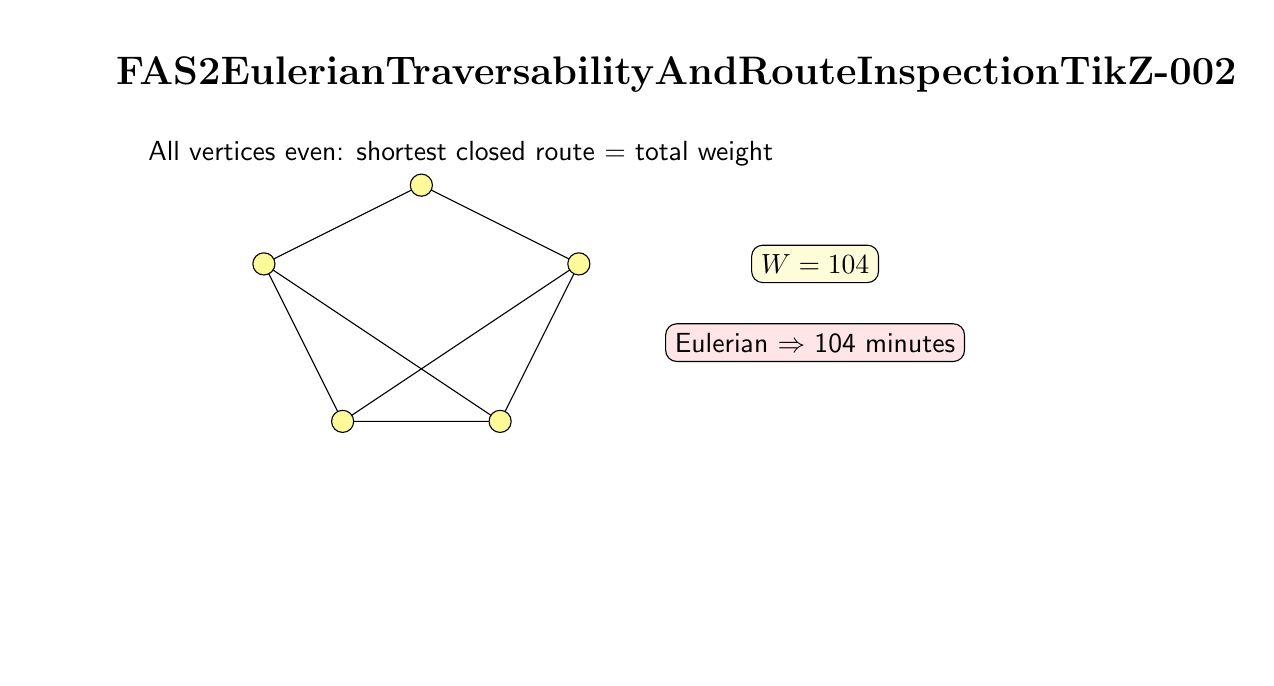
\begin{tikzpicture}[font=\sffamily]
\fill[white] (-1,-1) rectangle (13,7);
\node[anchor=west,font=\bfseries\Large] at (0,6.4) {FAS2EulerianTraversabilityAndRouteInspectionTikZ-002};

\node at (4.5,5.4) {All vertices even: shortest closed route = total weight};
\draw (2,4)--(4,5)--(6,4)--(5,2)--(3,2)--cycle (2,4)--(5,2) (3,2)--(6,4);
\foreach \x/\y in {2/4,4/5,6/4,5/2,3/2}{\filldraw[fill=yellow!40] (\x,\y) circle (4pt);}
\node[draw,rounded corners,fill=yellow!15] at (9,4) {$W=104$};
\node[draw,rounded corners,fill=red!10] at (9,3) {Eulerian $\Rightarrow$ 104 minutes};

\end{tikzpicture}
\end{document}
